\documentclass[tikz,10pt,a4paper]{article}
\usepackage{a4wide}
\usepackage[utf8]{inputenc}
\usepackage[T2A]{fontenc}
\usepackage{graphics,graphicx,epsfig}
\usepackage{amssymb,amsfonts,amsthm,amsmath,mathtext,cite,enumerate,float}
\usepackage[english,russian]{babel}
\usepackage[all]{xy}
\usepackage{morefloats}
\usepackage{pgf}
\usepackage[debug,outputdir={docgraphs/}]{dot2texi}
\usepackage{tikz}
\usepackage{scalefnt}
\usepackage{listings}
\usepackage{float}
\usepackage{verbatim}
\usepackage{placeins}
\usepackage{url}
\usepackage{babelbib}
\usepackage{pbox}
\usepackage{grffile}
\usepackage{color}
\usepackage{xfrac}
\usepackage{comment}
\usepackage{rotating}
\usepackage{slashbox}
\usepackage{caption}
\usepackage{subcaption}
\usetikzlibrary{arrows,shapes,intersections,decorations.markings,calc}

\makeatletter
\def\@settitle{\begin{center}%
    \baselineskip14\p@\relax
    \bfseries
    \@title
  \end{center}%
}

\makeatother

\newcommand{\bomega}{\boldsymbol{\omega}}

\begin{document}

\begin{center}
  МОДИФИКАЦИЯ ФУНКЦИОНАЛА ОШИБКИ В ЗАДАЧАХ НЕЛИНЕЙНОЙ РЕГРЕССИИ ДЛЯ УЧЕТА ПОГРЕШНОСТИ В ИЗМЕРЯЕМЫХ ДАННЫХ

  \bigskip
  Г.\,И.~Рудой
\end{center}

\begin{abstract}
  Рассматривается случай существенно нелинейной регрессионной зависимости
  в физическом эксперименте с гетероскедастичными погрешностями измерения
  как зависимых, так и независимых переменных.
  Предлагается модифицированный функционал среднеквадратичной ошибки,
  учитывающий погрешности определения независимых переменных и различные распределения
  погрешностей в разных точках. Рассматривается сходимость минимизирующего этот функционал
  вектора параметров к оптимальному для классического
  функционала среднеквадратичной ошибки.
  Приводятся результаты численного моделирования на данных, полученных в ходе
  эксперимента по измерению зависимости мощности лазера от прозрачности
  резонатора, показывающие преимущество предложенного функционала.

  \textbf{Ключевые слова}: \emph{гетероскедастичные ошибки,
  ошибки измерения независимых переменных, символьная регрессия, нелинейные модели.}
\end{abstract}

\section{Введение}

В ряде экспериментальных приложений возникает задача нахождения оптимальных
коэффициентов $\boldsymbol{\omega}$ некоторой регрессионной модели $f$, заданной
в виде аналитической формулы, по набору экспериментальных данных. Для этого
в предположении о нормальном распределении регрессионных остатков
строится функционал $\sum_i (y_i - f(x_i, \boldsymbol{\omega}))^2$,
представляющий сумму квадратов отклонений экспериментальных точек $y_i$ от
регрессионной кривой, и находится вектор параметров $\boldsymbol{\omega}$, его
минимизирующий.

Однако, данный функционал корректен только для точно измеренных независимых
переменных и гомоскедастичности ошибок измерения зависимой переменной. Иными
словами, предполагается существование лишь ошибок измерения зависимой
переменной, для которых дисперсия соответствующего распределения принимается
одинаковой.

В большинстве естественнонаучных приложений это предположение не выполняется,
особенно при измерении некоторой зависимости в достаточно широких диапазонах.
Например, в задаче нахождения зависимости коэффициента преломления $n$ прозрачного
полимера от длины волны $\lambda$ погрешности измерения каждого физического
параметра в различных точках, вообще говоря, различны\cite{Rudoy15MonteCarlo}.
Так, если для измерения длины волны $\lambda$ используется дифракционная
решетка, то постоянной является относительная погрешность определения длины волны
$\frac{\sigma_{\lambda_i}}{\lambda_i} \approx \text{const}$, и, следовательно,
погрешность определения длины волны зависит от самой длины волны. Подобная ситуация
фиксированной относительной (а не абсолютной) ошибки является типичной для
физических экспериментов.

Таким образом, возникает задача поиска оптимальных коэффициентов регрессионной
формулы с учетом отличающихся погрешностей измерения в различных экспериментальных точках.
Для некоторых частных случаев эта задача уже была решена.

Например, в \cite{jukic2013nonlinear} рассматривается модель Басса,
описывающая принятие и распространение новых потребительских продуктов в популяции
со временем, для которой вводится предположение о неравной точности измерений
в различных экспериментальных точках, что описывается различными весовыми коэффициентами при
соответствующих регрессионных остатках. При этом весовые коэффициенты имеют достаточно
общий вид и вводятся произвольно в виде экспертно указанных значений.

Другим примером является \cite{jukic2010nonlinear}, где рассматривается задача оценки коэффициентов
трехпараметрического распределения Вейбулла по неточно измеренным зависимым и
независимым данным. Для этого используется метод латентных переменных: к
независимым переменным $t_i$ добавляются <<свободные>> переменные $\delta_i$,
предоставляющие степень свободы в пространстве независимых переменных, и минимизируется
функционал вида
\[
  T(\alpha, \beta, \eta, \boldsymbol{\delta}) = \sum_{i = 0}^n w_i [f(t_i + \delta_i; \alpha, \beta, \eta) - y_i]^2 + \sum_{i = 0}^n p_i \delta_i^2,
\]
где $\alpha, \beta, \eta$~--- параметры распределения, а $w_i$ и $p_i$ являются
некоторыми экспертно заданными весами, соответствующими относительной точности
$i$-го измерения аналогично \cite{jukic2013nonlinear}.

В настоящей работе рассмотрена более общая ситуация, в которой не только зависимые,
но и независимые переменные определяются неточно, и каждая переменная
имеет свою собственную погрешность измерения. Исследуется случай
нелинейной регрессионной зависимости, в отличие от, например,
\cite{kiryati2000heteroscedastic}, изучающей линейную модель.

Предложен модифицированный функционал качества, учитывающий погрешности как
зависимых, так и независимых переменных в виде, достаточном для большинства
практических приложений. Весовые коэффициенты при регрессионных остатках
в настоящей работе выводятся из базовых предположений о распределении
погрешностей измерения и о поведении регрессионной модели в окрестности каждой
экспериментальной точки. На примере широко применяемого алгоритма
Левенберга-Марквардта\cite{Marquardt1963Algorithm} рассматривается модификация
имеющихся методов оптимизации, применяемых в подобных задачах (классический
и модифицированный алгоритмы будем в дальнейшем обозначать АЛМ и мАЛМ
соответственно). По построению показывается, что модифицированный алгоритм
оптимизации имеет те же свойства (например, скорость сходимости), что и
исходный алгоритм.
Приводятся результаты анализа экспериментальных данных по измерению параметров
усиливающей среды газового лазера. В рамках анализа, помимо непосредственного
нахождения коэффициентов регрессионной модели, сравнивалась сходимость
минимизирующих как предложенный, так и классический функционал параметров
к некоторым <<истинным>> значениям. Показано, что в подавляющем большинстве
рассмотренных случаев предложенный функционал дает лучшие приближения.

\section{Постановка задачи}

Дана обучающая выборка $D$:
\begin{equation}
  D = \{ \mathbf{x}_i, y_i \} | i \in \{ 1, \dots, \ell \}, \mathbf{x}_i \in \mathbb{R}^m, y_i \in \mathbb{R}.
  \label{eq:d}
\end{equation}
Для каждой зависимой переменной переменной $y_i$ известно
стандартное отклонение ошибки ее измерения $\sigma_{y_i}$, а для соответствующего
вектора независимых переменных $\mathbf{x}_i$ аналогично известны стандартные
отклонения его компонент $\sigma_{x_{ij}} | j \in \{ 1, \dots, m \}$.
Пусть, кроме того, выбрана некоторая регрессионная модель
$y = f (\mathbf{x}, \bomega)$, параметризованная вектором $\bomega$.

Для удобства введем вектор, составленный из ошибок измерений зависимых переменных
$\sigma_{y_i}$:
\[
  \boldsymbol{\sigma}_y = \{ \sigma_{y_1}, \dots, \sigma_{y_{\ell}} \}.
\]

Аналогично введем матрицу, составленную из ошибок измерений независимых переменных
$\sigma_{x_{ij}}$:
\[
  \Sigma_x = \| \sigma_{x_{ij}} \| | i \in \{ 1, \dots, \ell \}, j \in \{ 1, \dots, m \}.
\]

Требуется построить функционал ошибки $\breve{S}(\bomega)$ вектора параметров
$\bomega$ модели $f$, учитывающий ошибки измерений $\boldsymbol{\sigma}_y$ и
$\Sigma_x$:
\begin{equation}
  \breve{S}(\bomega) = \breve{S}(\bomega, \boldsymbol{\sigma}_y, \Sigma_x),
  \label{eq:s_modified}
\end{equation}
и, кроме того, найти вектор параметров $\omega$, минимизирующий функционал
\eqref{eq:s_modified}:
\begin{equation}
  \hat{\bomega} = \mathop{\arg \min}\limits_{\bomega} \breve{S}(\bomega).
\end{equation}

\section{Модифицированный функционал качества}

Воспользуемся следующим естественным качественным физическим соображением:
чем больше погрешность определения зависимой или независимых переменных
для некоторой экспериментальной точки, тем меньше соответствующий
регрессионный остаток должен учитываться при оптимизации параметров модели.
Кроме того, с физической точки зрения складывать
можно только величины, имеющие одинаковую размерность, либо безразмерные
величины, поэтому необходима соответствующая нормировка невязок по каждому из
измерений.

Сначала рассмотрим случай одной независимой переменной:
$x \in \mathbb{R}$. С учетом приведенных выше соображений введем
следующее определение расстояния $\rho(x, i)$
от точки $(x_i, y_i)$ до некоторой точки
$(x, f(x, \bomega))$ на кривой, описываемой регрессионной моделью $y = f(x, \bomega)$:
\begin{equation}
  \rho^2(x, i) = \frac{(x_i - x)^2}{\sigma_{x_i}^2} + \frac{(y_i - y)^2}{\sigma_{y_i}^2}.
  \label{eq:dist0}
\end{equation}

\begin{figure}[h]
  \centering
  \begin{tikzpicture}[
      scale = 1.5,
      point/.style = { draw, black, circle, fill, scale = 0.2 },
      classical/.style = { magenta },
      linearized/.style = { blue },
      ideal/.style = { orange },
      tangent/.style = {
        decoration = {
        markings,
        mark =
          at position #1
          with
          {
            \coordinate (tangent point-\pgfkeysvalueof{/pgf/decoration/mark info/sequence number}) at (0pt, 0pt);
            \coordinate (tangent unit vector-\pgfkeysvalueof{/pgf/decoration/mark info/sequence number}) at (1, 0pt);
            \coordinate (tangent orthogonal unit vector-\pgfkeysvalueof{/pgf/decoration/mark info/sequence number}) at (0pt, 1);
          }
        },
        postaction=decorate
      },
      use tangent/.style = {
        shift = (tangent point-#1),
        x = (tangent unit vector-#1),
        y = (tangent orthogonal unit vector-#1)
      },
      use tangent/.default = 1
    ]
    \coordinate (O) at (0,0);
    \draw[->, name path = Ox] (-0.3,0) -- (8,0) coordinate[label = { below:$x$ }] (xmax);
    \draw[->, name path = Oy] (0,-0.3) -- (0,6) coordinate[label = { right:$y$ }] (ymax);

    \draw[thick, red, tangent = 0.54, name path = f_x] plot[smooth] coordinates {(1, 4.875) (2, 4.75) (3, 4.5) (4, 4) (5, 3.1) (6, 1) (7, 1.5) };
    \node at (2, 5) {$f(x, \bomega)$};

    \draw[ideal, dashed, use tangent = 1] (-2, 0) -- (2, 0);
    \draw[ideal, use tangent = 1]
      (0, 0) node[point] (ideal_cp) {} --
      (0, 1.5) node[point, label = { [black]right:$(x_i, y_i)$ }] (datapt) {}
          node[pos = 0.6, label = { [black]below:$\tilde{\rho}$ }] {};

    \path[name path = vert_ideal_cp] (ideal_cp) -- ++ (270:5);
    \path[name path = hor_ideal_cp] (ideal_cp) -- ++ (180:5);
    \draw[ideal, dotted, name intersections = {of=vert_ideal_cp and Ox}]
      (ideal_cp) -- (intersection-1) node[point, label = { 275:$\tilde{x}$}] {};
    \draw[ideal, dotted, name intersections = {of=hor_ideal_cp and Oy}]
      (ideal_cp) -- (intersection-1) node[point, label = { left:$f(\tilde{x}, \bomega)$}] {};

    \path[name path = vertical_dp] (datapt) -- ++ (270:5);
    \draw[classical, name intersections = {of=f_x and vertical_dp, by={intersect}}]
      (datapt) --
      (intersect) node[point] (classical_cp) {}
          node[pos = 0.5, label = { [black]right:$y_i - f(x_i, \bomega)$ }] {};

    \path[name path = vert_classical_cp] (classical_cp) -- ++ (270:3);
    \path[name path = hor_classical_cp] (classical_cp) -- ++ (180:6);
    \draw[classical, dotted, name intersections = {of=vert_classical_cp and Ox}]
      (classical_cp) -- (intersection-1) node[point, label = { below:$x_i$ }] {};
    \draw[classical, dotted, name intersections = {of=hor_classical_cp and Oy}]
      (classical_cp) -- (intersection-1) node[point, label = { left:$f(x_i, \bomega)$ }] {};

    \path[name path = almost_vertical_dp] (datapt) -- ++ (271.5:5);
    \path[name intersections = {of=f_x and almost_vertical_dp}]
      (datapt) --
      (intersection-1) node[point, transparent] (almost_classical_cp) {};

    \draw[linearized, dashed, shorten >= -1cm, shorten <= -4cm] (classical_cp) -- (almost_classical_cp);

    \node[linearized, point] (linearized_orto) at ($(classical_cp)!(datapt)!(almost_classical_cp)$) {};
    \draw[linearized] (linearized_orto) -- (datapt)
          node[pos = 0.4, label = { [black]above:$\rho$ }] {};

    \path[name path = vert_linearized] (linearized_orto) -- ++ (270:5);
    \path[name path = hor_linearized] (linearized_orto) -- ++ (180:5);
    \draw[linearized, dotted, name intersections = {of=vert_linearized and Ox}]
      (linearized_orto) -- (intersection-1) node[point, label = { 265:$\hat{x}$ }] {};
    \draw[linearized, dotted, name intersections = {of=hor_linearized and Oy}]
      (linearized_orto) -- (intersection-1) node[point, label = { left:$\mathbb{L}_i[f](\hat{x}, \bomega)$ }] {};
  \end{tikzpicture}
  \caption{Различные способы определения расстояния от точки до прямой: $\tilde{\rho}$~---
    истинное расстояние как минимум расстояния от точки $(x_i, y_i)$ до какой-либо
    точки на прямой, $y_i - f(x_i, \boldsymbol{\omega})$~--- расстояние в классическом
    функционале среднеквадратичной ошибки в предположении об отсутствии ошибок измерения
    независимой переменной, $\rho$~--- предлагаемое нами расстояние.}
  \label{fig:distances}
\end{figure}

Непосредственное точное определение расстояния от экспериментальной
точки до регрессионной кривой представляется отдельной
сложной вычислительной задачей, однако в подавляющем большинстве
практических приложений регрессионные зависимости достаточно
гладкие, а погрешности измерения достаточно малы. При этих предположениях
будем рассматривать расстояние не от точки до кривой, а от точки до
линеаризованной в окрестности этой точки кривой. Так, на рис. \ref{fig:distances}
показаны различные варианты определения расстояния, при этом
в иллюстративных целях размерности и погрешности определения $x$ и $y$ приняты
одинаковыми.

Итак, линеаризуем $f(x, \bomega)$ в окрестности точки $(x_i, f(x_i, \bomega))$,
обозначив оператор линеаризации в окрестности этой точки как $\mathbb{L}_i$:
\begin{equation}
  f(x, \bomega) \approx \mathbb{L}_{i}[f](x, \bomega) = f(x_i, \bomega) + (x - x_i) \frac{\partial f}{\partial x}(x_i, \bomega),
  \label{eq:f_linear}
\end{equation}
Расстояние \eqref{eq:dist0} выражается для линеаризованной функции
\eqref{eq:f_linear} следующим образом:
\begin{equation}
  \rho^2(x, i) = \frac{(x_i - x)^2}{\sigma_{x_i}^2} + \frac{(y_i - f(x_i, \bomega) - \frac{\partial f}{\partial x}(x_i, \bomega) (x - x_i))^2}{\sigma_{y_i}^2}.
  \label{eq:dist_linear}
\end{equation}
Минимизируя это выражение по $x$:
\[
  \hat{x} = \mathop{\arg \min}\limits_x \rho^2(x, i),
\]
находим расстояние от точки $(x_i, y_i)$ из обучающей выборки до
линеаризованной в ее окрестности регрессионной зависимости $f$ при
данном векторе параметров $\bomega$:
\begin{equation}
  \rho^2(f, \bomega, i) = \rho^2(\hat{x}, i) = \frac{(y_i - f(x_i, \bomega))^2}{\sigma^2_{y_i} + \frac{\partial f}{\partial x}(x_i, \bomega)^2 \sigma^2_{x_i}}.
  \label{eq:rho_univar}
\end{equation}

Аналогично можно получить выражение для случая, когда объекты в обучающей выборке
представлены $m$ независимыми переменными ($\mathbf{x} \in \mathbb{R}^m$).
Таким образом, предлагаемый нами функционал, минимизирующий сумму введеных согласно \eqref{eq:dist0}
расстояний, для достаточно гладких функций выглядит следующим образом:
\begin{equation}
  \breve{S}(\bomega) = \sum_{i = 1}^\ell \frac{(y_i - f(\mathbf{x}_i, \bomega))^2}{\sigma_{y_i}^2 + \sum_{j = 1}^m (\frac{\partial f}{\partial x_j}(\mathbf{x}_i, \bomega))^2 \sigma^2_{x_{ij}}}.
  \label{eq:s}
\end{equation}

Отметим следующее:
\begin{itemize}
  \item Функционал \eqref{eq:s} соответствует классической сумме квадратов регрессионных
	остатков при условии нормировки квадрата каждого остатка на сумму квадратов погрешности
	определения зависимой величины $\sigma_{y_i}$ и произведения частной производной
	регрессионной модели по $j$-ой компоненте вектора независимых величин на погрешность
	определения соответствующей компоненты $\sigma_{x_{ij}}$.

  \item При прочих равных условиях в выражении для расстояния \eqref{eq:rho_univar} и,
	соответственно, в функционале \eqref{eq:s} с большим весом учитываются те точки, в которых
	производная регрессионной модели $\frac{\partial f}{\partial x_j}$ по соответствующей
	компоненте $x_j$ больше, что соответствует соображениям здравого смысла: чем меньше наклон
	регрессионной зависимости в окрестности данной точки, тем меньше влияние неточного
	измерения соответствующей независимой переменной на значение регрессионной зависимости
	в этой точке.

  \item Если все независимые переменные измерены точно, то есть,
	$\forall i, j : \sigma_{x_{ij}} = 0$, то предложенный функционал переходит в рассмотренный
	в \cite{jukic2013nonlinear}. Если же, кроме того, все зависимые переменные имеют одну и ту же погрешность,
	то предложенный функционал переходит в известную сумму квадратов регрессионных остатков
	с точностью до некоторого множителя $\sigma_y$, не влияющего на положения минимумов функционала
	среднеквадратичной ошибки.
\end{itemize}

\section{Метод оптимизации предложенного функционала}

Для численной оптимизации функционала \eqref{eq:s} представим его в виде
суммы квадратов регрессионных остатков путем следующего переобозначения переменных.
Вместо выборки \eqref{eq:d}
рассмотрим выборку
\[
  \tilde{D} = \{ \tilde{\mathbf{x}}_i, \tilde{y}_i \} | i \in \{ 1, \dots, \ell \}, \tilde{\mathbf{x}}_i \in \mathbb{R}^{m + 1}, y_i \in \mathbb{R},
\]
где $\tilde{y}_i \equiv 0$, а
$\tilde{\mathbf{x}}_i = \{ \mathbf{x}_i, y_i \}$~--- исходный вектор $\mathbf{x}_i$
с дополнительно приписанным к нему значением $y_i$. Кроме того, примем
\[
  \tilde{f}(\tilde{\mathbf{x}}_i, \bomega) = \frac{f(\mathbf{x}_i, \bomega) - y_i}{\sqrt{\sigma_{y_i}^2 + \sum_{j = 1}^m (\frac{\partial f}{\partial x_j}(\mathbf{x}_i, \bomega))^2 \sigma^2_{x_{ij}}}}.
\]
Тогда минимизация функционала \eqref{eq:s} возможна известными методами оптимизации, так
как легко видеть, что \eqref{eq:s} в этом случае эквивалентен
\[
  S(\bomega) = \sum_{i = 1}^\ell (\tilde{y}_i - \tilde{f}(\tilde{\mathbf{x}}_i, \bomega))^2.
\]

\begin{comment}
Легко показать, что градиент $\tilde{f}$ по параметрам выглядит следующим образом:
\begin{footnotesize}
\[
  \frac{\partial\tilde{f}}{\partial \omega_k}(\mathbf{x}_i, \bomega) = \frac{
		\frac{\partial f}{\partial \omega_k}(\mathbf{x}_i, \bomega) \Big(\sigma_{y_i}^2 + \sum_{j = 1}^m \big(\frac{\partial f}{\partial x_j} (\mathbf{x}_i, \bomega)\big)^2 \sigma_{x_{ij}}^2 \Big)-
		\big(f(\mathbf{x}_i, \bomega) - y_i\big) \sum_{j = 1}^m \sigma_{x_{ij}}^2 \frac{\partial f}{\partial x_j}(\mathbf{x}_i, \bomega) \frac{\partial^2 f}{\partial x_j \partial \omega_k}(\mathbf{x}_i, \bomega)}
  {\Big( \sigma_{y_i}^2 + \sum_{j = 1}^m \big(\frac{\partial f}{\partial x_j} (\mathbf{x}_i, \bomega)\big)^2 \sigma_{x_{ij}}^2 \Big)^{\sfrac{3}{2}}}.
\]
\end{footnotesize}
\end{comment}

Как видно из построения, в качестве базового алгоритма оптимизации может
быть использован любой метод решения задачи о наименьших квадратах, как, например,
метод градиентного спуска или алгоритм Левенберга-Марквардта\cite{dlib09}. Кроме того, при
соответствующих условиях гладкости частных производных функции $f$ (что практически
всегда выполняется в реальных физических приложениях) сохраняются все свойства
исходного алгоритма.

Отметим, что предложенная идея введения весовых коэффициентов, отвечающих различным
измерениям и зависящих от точности этих измерений, вообще говоря применима и для
прочих методов решения задачи восстановления регрессии, отличных от символьной регрессии.
Подробное рассмотрение этих методов в совокупности с данной идеей выходит за рамки
данной статьи, однако отметим, что при невозможности выполнить аналитическое
дифференцирование функции $f$ предлагается использовать следующий
следующий итеративный алгоритм, предназначенный для использования с уже имеющимися
реализациями методов оптимизации. Предполагается, что соответствующая реализация
<<принимает на вход>> массив значений $y_i$,
функцию вычисления значения $f$ в точках $\mathbf{x}_i$ с вектором параметров $\bomega$,
и критерий останова в виде числа итераций.

Алгоритм выглядит следующим образом:
\begin{enumerate}
  \item Выбирается некоторое начальное приближение вектора параметров $\bomega$.
  \item Для каждой пары $(\mathbf{x}_i, y_i)$ из обучающей выборки численно или
	аналитически рассчитывается значение частной производной
	$\frac{\partial f}{\partial x}$ в точке $(\mathbf{x}_i, \bomega)$.
  \item Каждое значение зависимой переменной $y_i$ и значение функции $f(\mathbf{x}_i, \bomega)$
	нормируется на соответствующую величину
	\[
	  \sigma_{y_i}^2 + \sum_{j = 1}^m (\frac{\partial f}{\partial x_j}(\mathbf{x}_i, \bomega))^2 \sigma^2_{x_{ij}}.
	\]
  \item Выполняется итерация классического алгоритма оптимизации для таким образом
	модифицированных значений функции $f$ и зависимых переменных $y_i$, таким образом
	получается новое значение вектора $\bomega$.
  \item Если критерий останова не достигнут, алгоритм продолжает выполнение с пункта 2.
\end{enumerate}

Отметим следующее:
\begin{itemize}
  \item Критерием останова могут служить обычные критерии вроде достижения некоторого
    числа итераций, нормы изменения вектора $\bomega$, и т.~п.
  \item Если известно, что производная $\frac{\partial f}{\partial x}$ является достаточно гладкой
	в окрестности $(\mathbf{x}_i, \bomega) \mid i \in \{ 1, \dots, \ell \}$, на шаге
	4 алгоритма представляется разумным выполнить сразу несколько итераций
	классического алгоритма во избежание потенциально ресурсоемкого пересчета производных и
	перенормировки значений $y_i$ и $f$.
\end{itemize}

\section{Вычислительный эксперимент}

В вычислительном эксперименте рассматриваются данные, полученные в ходе измерения
зависимости интенсивности излучения $I$ лазера от прозрачности его резонатора.
Изучался лазер высокого давления ($\approx 3\ \text{атм}\ He, \approx 60\ \text{Торр}\ Ne, \approx 20\ \text{Торр}\ Ar$) на
$3p-3s$ переходах неона (основной переход~--- 585 нм), возбуждаемый электронным пучком\cite{alexandrov1991kinetics}.

Пусть насыщающая переход интенсивность излучения~--- $I_s$, наблюдаемая интенсивность~---
$I_l$. В таком случае для безразмерной величины $y = \frac{I_l}{I_s}$ с учетом однородного
уширения линии усиления при высоком давлении газа и хорошей однородности возбуждения,
обеспечиваемой электронным пучком, можно получить нелинейное уравнение \cite{champagne1982transient}:
\begin{equation}
  \alpha_0 L - \frac{1}{2} \ln R_0 = g_0 L \frac{1 + \sqrt{R_0}}{1 - \sqrt{R_0}} \frac{1}{y} \ln \Big( 1 + \frac{y \frac{1 - \sqrt{R_0}}{1 + \sqrt{R_0}}}{1 + y \frac{2 \sqrt{R_0}}{1 - R_0}} \Big),
  \label{eq:y_exact}
\end{equation}
где $\alpha_0$~--- распределенные потери (например, на рассеяние света),
$g_0$~--- коэффициент усиления слабого сигнала, $R_0$~--- коэффициент отражения выходного
зеркала лазера. Однородность накачки означает, что $g_0$ и $\alpha_0$ одинаковы по
всему объему с хорошей точностью.

Значение $R_0$ является независимой переменной, изменяемой экспериментаторами, и в данном
разделе также обозначается $x$ сообразно остальной части работы.

Для достаточно больших $R_0$, близких к единице (фактически для $R_0 \geq 0.6 \div 0.7$),
можно упростить \eqref{eq:y_exact}, заменив $2 \sqrt{R_0} \approx 1 + R_0$ и получив
хорошо известное выражение:
\begin{equation}
  y(R_0) = \gamma \frac{1 - R_0}{1 + R_0} \Big(\frac{g_0}{\alpha_0 - \frac{1}{2} L \ln R_0} - 1\Big),
  \label{eq:y_approx}
\end{equation}
где $\gamma$~--- нормировочный коэффициент.

Длина активной среды $L$~--- 150 см, точность определения мощности лазера $y$ имеет
относительную погрешность в $2\%$, точность определения прозрачности $R_0$ имеет
абсолютную погрешность и составляет $0.01$ при $R_0 \geq 0.6$ и $0.02$ при $R_0 < 0.6$.

В ходе измерений получены значения $y(R_0)$, приведенные в таблице \ref{tabl:measurements}.

\begin{table}[h]
  \caption{Экспериментальные значения $y(R_0)$.}
  \centering
  \begin{tabular}{| r | r | r | r | r | r | r | r |}
	\hline
	$R_0$	&	0.48	&	0.56	&	0.65	&	0.73	&	0.80	&	0.87	&	0.94	\\ \hline
	$y$		&	3.25	&	10.2	&	16.5	&	20.5	&	22.5	&	23.2	&	18.2	\\ \hline
  \end{tabular}
  \label{tabl:measurements}
\end{table}

Таким образом, решается задача минимизации функционала \eqref{eq:s} при
\[
  \boldsymbol{\omega} = (\omega_1, \omega_2, \omega_3) = (\gamma, \alpha_0, g_0),
\]
\[
  f(x, \boldsymbol{\omega}) = y(R_0, \gamma, \alpha_0, g_0),
\]
\begin{equation}
  \begin{array}{ll}
	\sigma_{y_i} &= 0.02 y_i,\\
	\sigma_{x_i} &= \left\{
	  \begin{array}{lr}
		0.01 & \mid x_i \geq 0.6, \\
		0.02 & \mid x_i < 0.6.
	  \end{array}
	\right.
  \end{array}
  \label{eq:sigmas_definition}
\end{equation}

\subsection{Оптимальные параметры модели}
Кроме предложенного в настоящей работе функционала \eqref{eq:s} рассмотрен
также и классический функционал среднеквадратичной ошибки:
\begin{equation}
  S = \sum_{i = 1}^\ell (y_i - f(x_i, \boldsymbol{\omega}))^2,
  \label{eq:s_classic}
\end{equation}

В таблице \ref{tabl:res_coeffs} приведены значения параметров $\bomega$ и $\bomega^0$
функции \eqref{eq:y_approx},
минимизирующие \eqref{eq:s} и \eqref{eq:s_classic} соответственно, а также относительные
разности их компонент. Кроме того, приведены значения функционалов \eqref{eq:s} и
\eqref{eq:s_classic} для обоих векторов параметров.

\begin{table}[h]
  \caption{Оптимальные значения параметров модели.}
  \centering
  \begin{tabular}{| r | r | r | r | r | r | r | r | r |}
	\hline
													& $g_0$					& $\alpha_0$			& $\gamma$				& Значение \eqref{eq:s} & Значение \eqref{eq:s_classic}	\\ \hline
	$\bomega$										& $2.920 \cdot 10^{-3}$	& $2.156 \cdot 10^{-4}$	& $100.324$				& $0.577$				& $0.208$						\\ \hline
	$\bomega^0$										& $2.917 \cdot 10^{-3}$	& $2.129 \cdot 10^{-4}$	& $101.5$				& $0.645$				& $0.183$						\\ \hline
	$\sfrac{|\omega_i - \omega^0_i|}{\omega^0_i}$	& $1.03 \cdot 10^{-3}$	& $1.27 \cdot 10^{-2}$	& $1.16 \cdot 10^{-2}$	& $0.11$				& $0.14$						\\ \hline
  \end{tabular}
  \label{tabl:res_coeffs}
\end{table}

Отдельно отметим, что сравнивать непосредственные значения функционалов \eqref{eq:s} и
\eqref{eq:s_classic} не имеет смысла. Вместо этого необходимо сравнивать различные
модели по каждому из этих функционалов в отдельности. Так, результаты, приведенные
в таблице \ref{tabl:res_coeffs}, показывают вполне естественный результат: каждый
из двух векторов параметров ($\bomega$ и $\bomega^0$) является оптимальным лишь
для того функционала, который он минимизирует.

Графики модели \eqref{eq:y_approx}, соответствующие $\bomega$ и $\bomega^0$, приведены
на рис. \ref{fig:results}.

\begin{figure}[h]
  \centering
  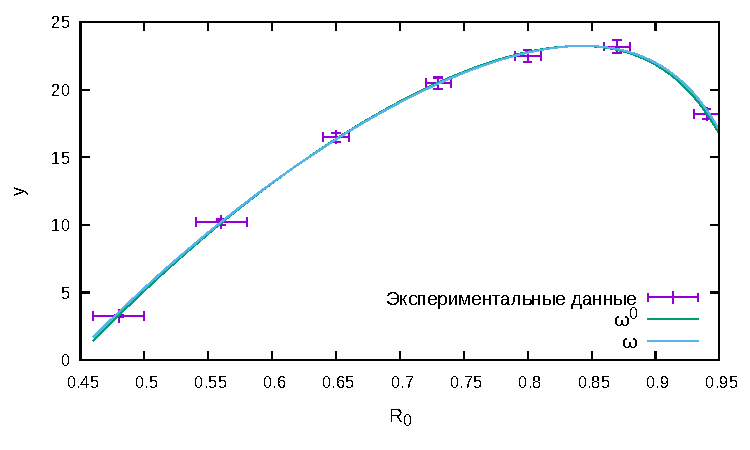
\includegraphics[width=0.8\textwidth]{figs/levmar/results.pdf}
  \caption{Графики \eqref{eq:y_approx}, соответствующие параметрам,
	минимизирующим \eqref{eq:s} и \eqref{eq:s_classic}.}
  \label{fig:results}
\end{figure}

\subsection{Сходимость оптимальных параметров к классическим}
Численно исследована зависимость сходимости параметров $\bomega$ к параметрам $\bomega^0$,
получаемым минимизацией функционалов \eqref{eq:s} и \eqref{eq:s_classic} соответственно, от
погрешности $\mathbf{\sigma}_y$ измерения зависимой переменной $y$.

Разумно ожидать, что при увеличении погрешности измерения величины $y$ при
фиксированной погрешности измерения $R_0$ оптимальный вектор $\boldsymbol{\omega}$
будет приближаться к $\boldsymbol{\omega}^0$, так как тем более незначителен
вклад ошибки измерения независимой переменной.

Рассматриваются два случая:
\begin{enumerate}
  \item Погрешность $i$-го измерения $y_i$ задается как $\sigma_{y_i} = 0.02ky_i$, т. е.
	погрешность зависит от значения самого $y_i$.
  \item Погрешность $i$-го измерения $y_i$ задается как $\sigma_{y_i} = 0.02ky_{\max}$,
	т. е. погрешность от значения конкретного $y_i$ не зависит. Заметим, что выбор
	конкретного значения $y$, определяющего погрешность, является в данном случае
	достаточно произвольным и соответствует умножению всех погрешностей на некоторую константу.
\end{enumerate}

В первом случае ошибки измерения $y$ распределены неодинаково, следовательно, применение
стандартного метода наименьших квадратов не обосновано. В то же время во втором случае
ошибки принадлежат одному и тому же распределению, и, кроме того, независимы, поэтому
в данном случае МНК-оценка применима (с точностью до ошибки измерения независимой
переменной).

Для обоих случаев подробно рассматривалась область $k \in [1; 100]$, значение $k$
изменялось с шагом 0.01. Отметим, что уже при $k \approx 25$ характерная погрешность
измерения величины $y$ сопоставима с самой величиной $y$, а при $k > 50$ превышает ее.

Результаты приведены на рис. \ref{fig:conv_varY}.
На графиках отображены компоненты вектора $\boldsymbol{\omega}$, нормированные на
соответствующие значения $\boldsymbol{\omega}^0$, в зависимости от значения $k$.

\begin{figure}[h]
  \centering
  \begin{subfigure}[b]{0.5\textwidth}
    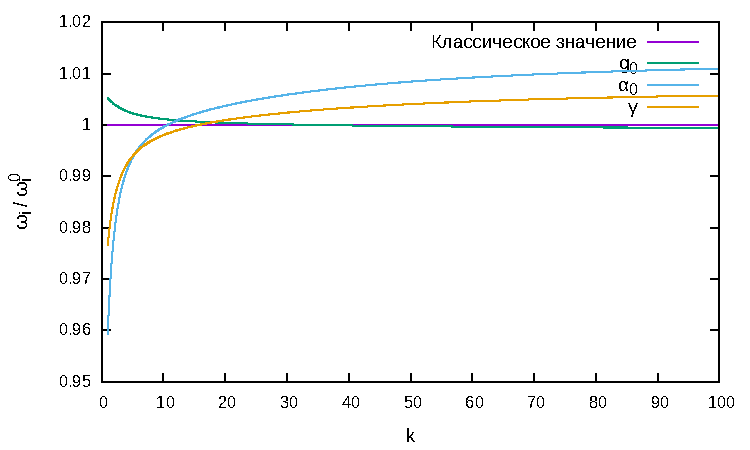
\includegraphics[width=\textwidth]{figs/levmar/convergence/varY/convergence_100.txt.pdf}
	\caption{$\sigma_{y_i} = 0.02ky_i$}
	\label{fig:conv_varY_100}
  \end{subfigure}%
  \begin{subfigure}[b]{0.5\textwidth}
    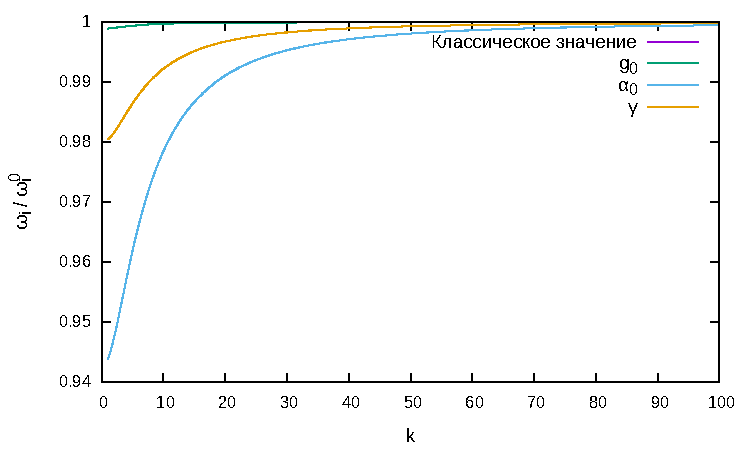
\includegraphics[width=\textwidth]{figs/levmar/convergence/fixedXY_0.1/convergence_100.txt.pdf}
	\caption{$\sigma_{y_i} = 0.02ky_{\max}$}
	\label{fig:conv_fixedY_100}
  \end{subfigure}
  \caption{Зависимость оптимальных параметров от $k \in [1; 100]$.}
  \label{fig:conv_varY}
\end{figure}

Видно, что в случае фиксированной погрешности $\sigma_{y_i}$ значения $\boldsymbol{\omega}$
действительно стремятся к $\boldsymbol{\omega}^0$ для разумных значений $k$, а в случае
гетероскедастичности ошибки такой зависимости не наблюдается, хотя значения $\boldsymbol{\omega}$
и оказываются достаточно близки к $\boldsymbol{\omega}^0$.

\subsection{Сходимость параметров к истинным}
Численно исследована зависимость сходимости параметров $\bomega = \arg \min \breve{S}$
и $\bomega^0 = \arg \min S$ к некоторому <<истинному>> значению вектора параметров
$\hat{\bomega}$, от количества точек $\ell$ в обучающей выборке и от погрешности определения
независимой переменной.

Для этого вектор параметров $\bomega$, полученный минимизацией обучающей выборки из таблицы
\ref{tabl:measurements}, принимается за некоторый <<истинный>> вектор параметров $\hat{\bomega}$,
и на каждой $j$-й итерации генерируется обучающая выборка $D_j(\ell, k)$:
\[
  D_j(\ell, k) = \{ (x_i + \xi^x_i, y(x_i, \hat{\bomega}) + \xi^y_i) \} \mid \xi^x_i \sim \mathcal{N}(0, k \sigma_{x_i}), \xi^y_i \sim \mathcal{N}(0, \sigma_{y_i}), i \in \{ 1, \dots, \ell \},
\]
где $y(x, \bomega)$ задано соотношением \eqref{eq:y_approx}, а $\sigma_{x_i}$ и $\sigma_{y_i}$
определяются соотношением \eqref{eq:sigmas_definition}.

Иными словами, генерируется обучающая выборка согласно искомой функции зависимости с
известным и фиксированным вектором параметров, которая затем зашумляется нормально
распределенным шумом. При этом стандартное отклонение шума для зависимой величины
совпадает с экспертно предложенным для реального эксперимента, а стандартное отклонение
независимой величины отличается от экспертно предложенного в $k$ раз.

После генерации выборки $D_j(\ell, k)$ по ней находятся значения $\bomega_j = \arg \min \breve{S}$
и $\bomega_j^0 = \arg \min S$, что повторяется $N$ раз, и рассматриваются значения
\[
  \overline{\delta \bomega} = \frac{\sum_{j = 1}^N \text{Abs}(\bomega_j - \hat{\bomega})}{N},
\]
\[
  \overline{\delta \bomega^0} = \frac{\sum_{j = 1}^N \text{Abs}(\bomega^0 - \hat{\bomega})}{N},
\]
где $\text{Abs}$ выполняет операцию взятия модуля над каждой компонентой аргумента-вектора: $\text{Abs}(\{ \omega_i \}) = \{ | \omega_i | \}$.

Иными словами, $\overline{\delta \bomega}$~--- вектор, компоненты которого представляют
среднее отклонение соответствующих компонент минимизирующего \eqref{eq:s} вектора от
$\hat{\bomega}$. Аналогично для $\overline{\delta \bomega}$ и \eqref{eq:s_classic}.

Таким образом, варьируя $k$ и изучая поведение $\overline{\delta \bomega}$ и $\overline{\delta \bomega^0}$, можно исследовать влияние погрешности определения
независимой переменной на разность между $\hat{\bomega}$ и оптимальными параметрами $\bomega$ и $\bomega^0$
согласно \eqref{eq:s} и \eqref{eq:s_classic} соответственно.

Так как при уменьшении $k$ монотонно уменьшается погрешность определения независимой
переменной, естественно ожидать, что различие между $\bomega$ и $\bomega^0$ будет
уменьшаться. Однако, наш вычислительный эксперимент демонстрирует, что это не так.

В нашем эксперименте $N = 1000$, $\ell \in \{ 10, \dots, 1000 \}$,
$k \in \{ 0.5, 0.6, 0.7, 0.8, 0.9, 1.0, 1.2, 1.4, 2, 3, \dots, 9 \}$.

Наиболее характерные результаты эксперимента приведены на рис.
\ref{fig:comparison_0.5}-\ref{fig:comparison_9}.

Стоит отметить следующее:
\begin{itemize}
  \item Во всех случаях предложенный в настоящей работе функционал \eqref{eq:s}
	дает лучшее приближение при разумно малом объеме обучающей выборки. Кроме того, в
	подавляющем большинстве случаев предпочтительность предложенного функционала
	сохраняется и для большего числа экспериментальных точек.
  \item Для малых $k \approx 0.5$ ошибка оценки параметров $\alpha_0$ и $\gamma$
	при помощи классического функционала \eqref{eq:s_classic}
	имеет ярко выраженный минимум в окрестности 60-100 экспериментальных точек
	(рис. \ref{fig:comparison_0.5_alpha} и \ref{fig:comparison_0.5_gamma}).
	Дальнейшее увеличение обучающей выборки ведет к ухудшению приближения, получаемого
	минмизацией \eqref{eq:s_classic}.
  \item Для некоторых $k$ ошибка приближения, получаемого минимизацией предложенного
	функционала \eqref{eq:s}, имеет явную горизонтальную асимптоту (рис. \ref{fig:comparison_0.5_alpha},
	\ref{fig:comparison_1}, \ref{fig:comparison_1.2_alpha} и \ref{fig:comparison_9_alpha}).
\end{itemize}

Вопрос о причинах подобного поведения оптимальных параметров является предметом
дальнейшей работы.

\begin{figure}[h]
  \centering
  \begin{subfigure}[b]{0.35\textwidth}
    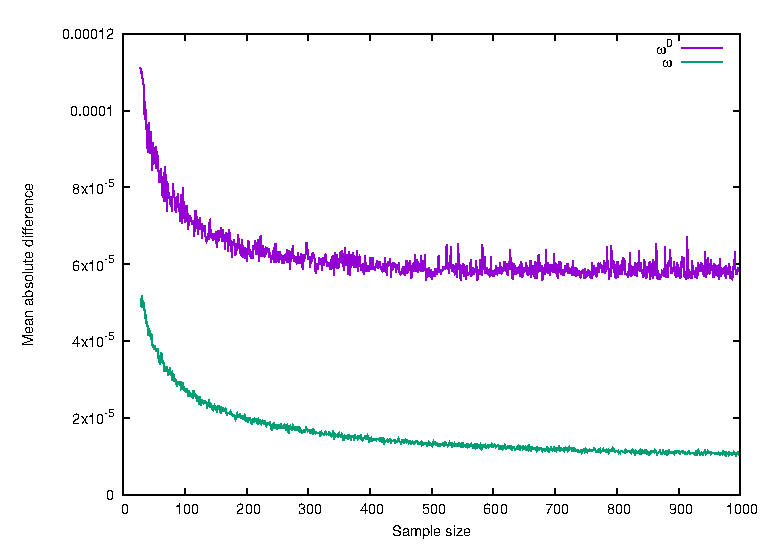
\includegraphics[width=\textwidth]{figs/levmar/comparison/comparison_1000_32_1000_xsigma0.5.txt_parameter1.eps}
	\caption{$g_0$}
  \end{subfigure}%
  \begin{subfigure}[b]{0.35\textwidth}
    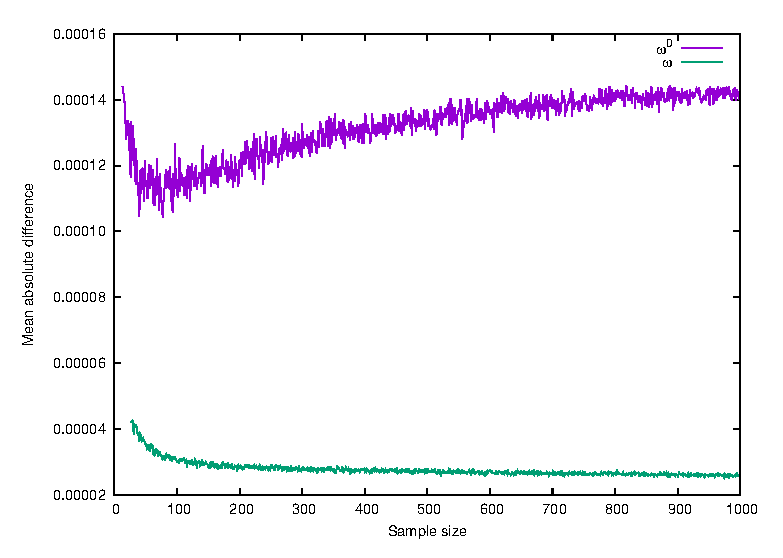
\includegraphics[width=\textwidth]{figs/levmar/comparison/comparison_1000_32_1000_xsigma0.5.txt_parameter2.eps}
	\caption{$\alpha_0$}
	\label{fig:comparison_0.5_alpha}
  \end{subfigure}%
  \begin{subfigure}[b]{0.35\textwidth}
    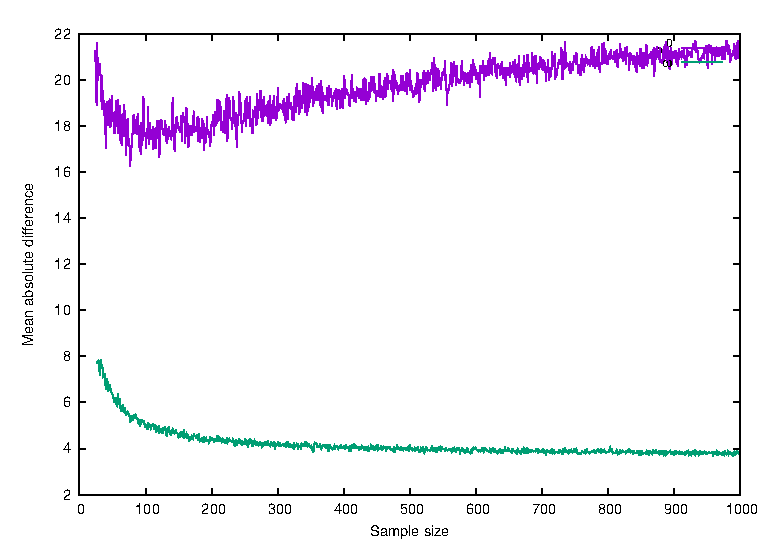
\includegraphics[width=\textwidth]{figs/levmar/comparison/comparison_1000_32_1000_xsigma0.5.txt_parameter3.eps}
	\caption{$\gamma$}
	\label{fig:comparison_0.5_gamma}
  \end{subfigure}
  \caption{Сходимость параметров к истинным при $k = 0.5$.}
  \label{fig:comparison_0.5}
\end{figure}

\begin{figure}[h]
  \centering
  \begin{subfigure}[b]{0.35\textwidth}
    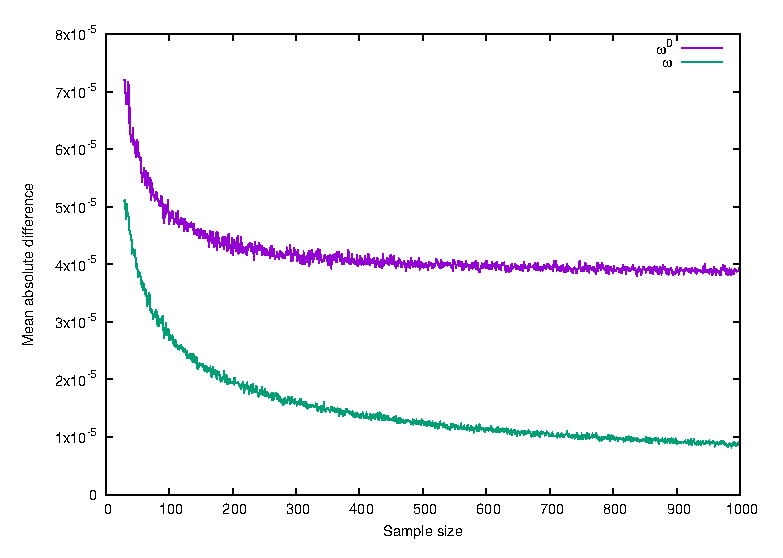
\includegraphics[width=\textwidth]{figs/levmar/comparison/comparison_1000_32_1000_xsigma0.8.txt_parameter1.eps}
	\caption{$g_0$}
  \end{subfigure}%
  \begin{subfigure}[b]{0.35\textwidth}
    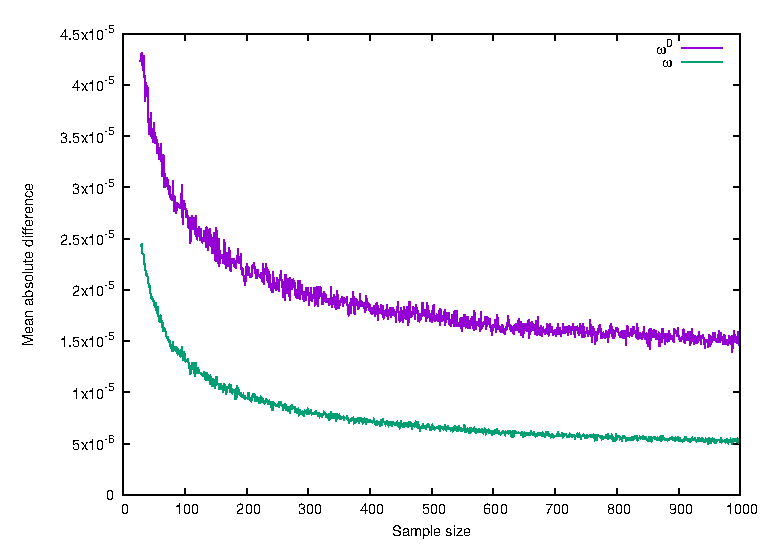
\includegraphics[width=\textwidth]{figs/levmar/comparison/comparison_1000_32_1000_xsigma0.8.txt_parameter2.eps}
	\caption{$\alpha_0$}
  \end{subfigure}%
  \begin{subfigure}[b]{0.35\textwidth}
    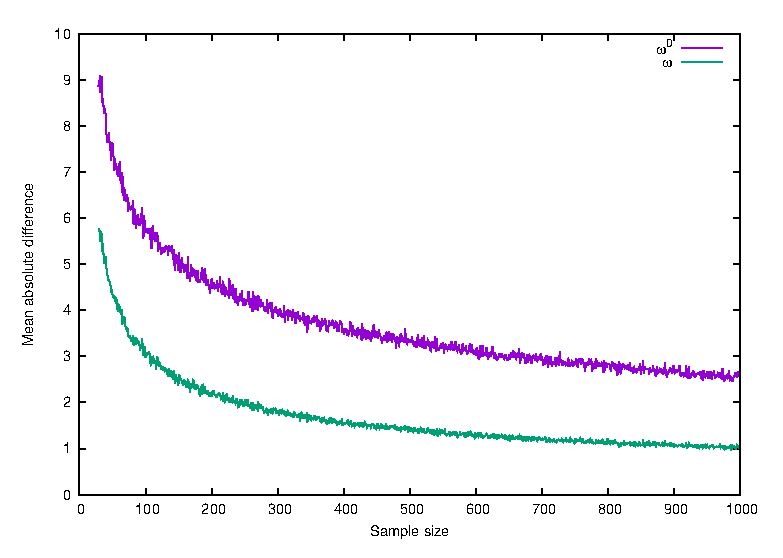
\includegraphics[width=\textwidth]{figs/levmar/comparison/comparison_1000_32_1000_xsigma0.8.txt_parameter3.eps}
	\caption{$\gamma$}
  \end{subfigure}
  \caption{Сходимость параметров к истинным при $k = 0.8$.}
  \label{fig:comparison_0.8}
\end{figure}

\begin{figure}[h]
  \centering
  \begin{subfigure}[b]{0.35\textwidth}
    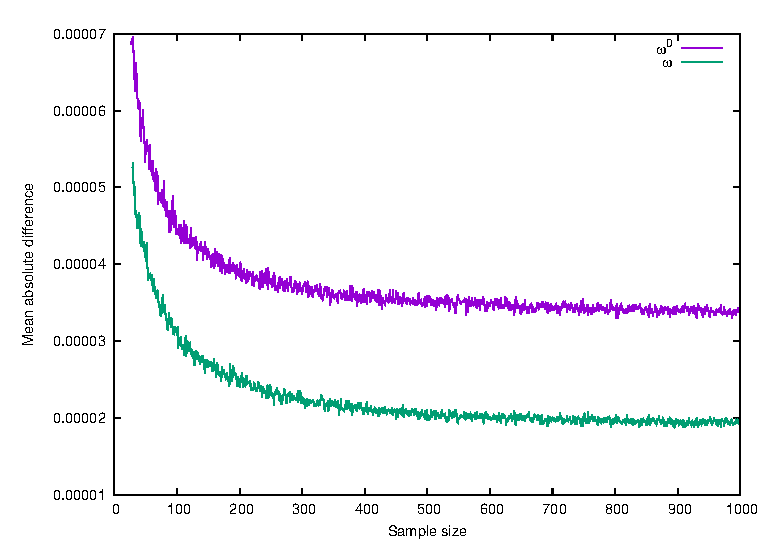
\includegraphics[width=\textwidth]{figs/levmar/comparison/comparison_1000_32_1000_xsigma0.9.txt_parameter1.eps}
	\caption{$g_0$}
  \end{subfigure}%
  \begin{subfigure}[b]{0.35\textwidth}
    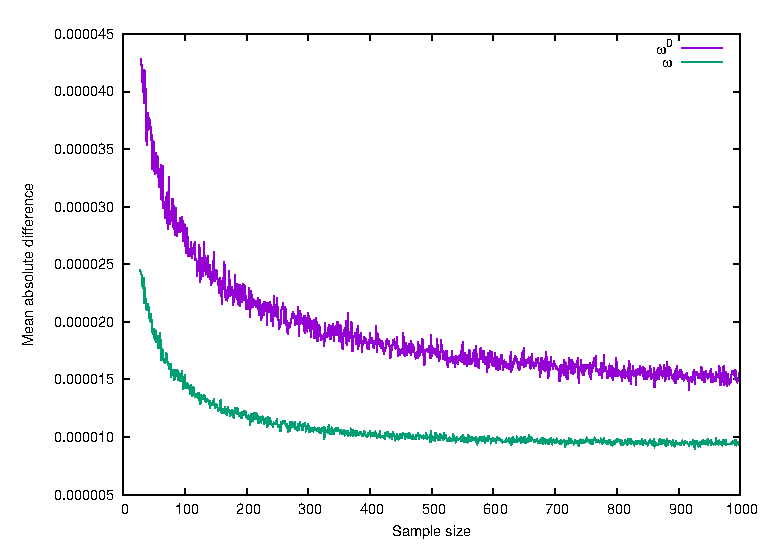
\includegraphics[width=\textwidth]{figs/levmar/comparison/comparison_1000_32_1000_xsigma0.9.txt_parameter2.eps}
	\caption{$\alpha_0$}
  \end{subfigure}%
  \begin{subfigure}[b]{0.35\textwidth}
    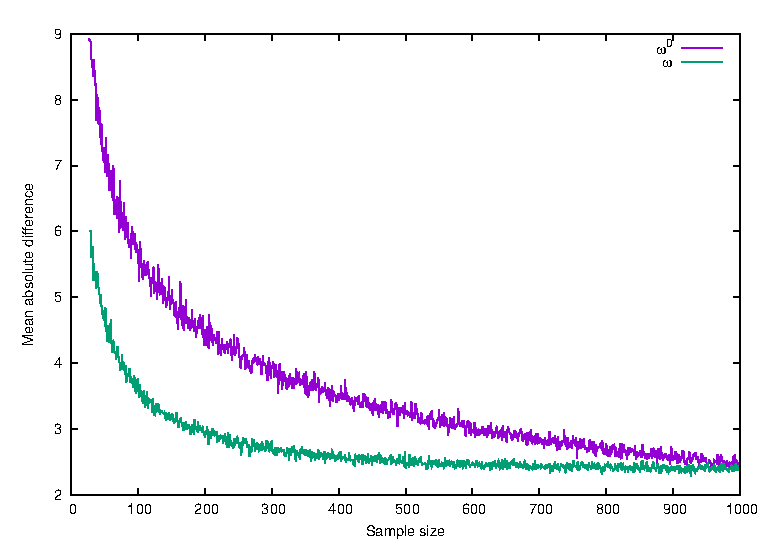
\includegraphics[width=\textwidth]{figs/levmar/comparison/comparison_1000_32_1000_xsigma0.9.txt_parameter3.eps}
	\caption{$\gamma$}
  \end{subfigure}
  \caption{Сходимость параметров к истинным при $k = 0.9$.}
  \label{fig:comparison_0.9}
\end{figure}

\begin{figure}[h]
  \centering
  \begin{subfigure}[b]{0.35\textwidth}
    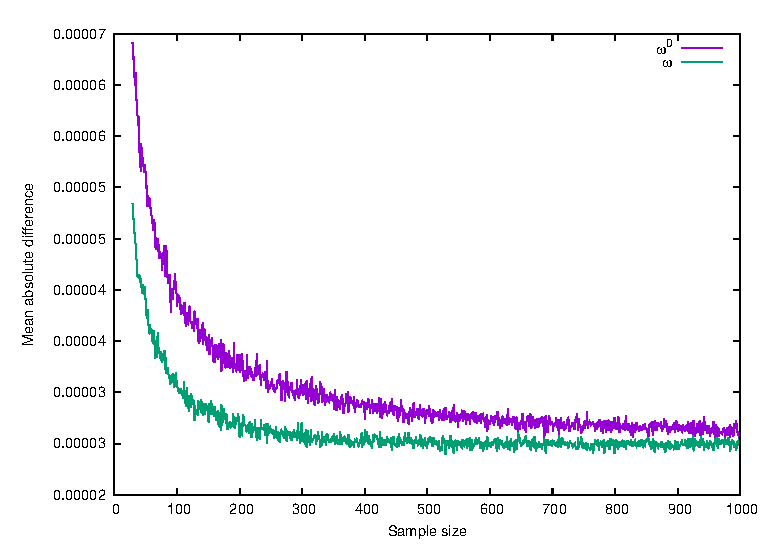
\includegraphics[width=\textwidth]{figs/levmar/comparison/comparison_1000_32_1000_xsigma1.txt_parameter1.eps}
	\caption{$g_0$}
  \end{subfigure}%
  \begin{subfigure}[b]{0.35\textwidth}
    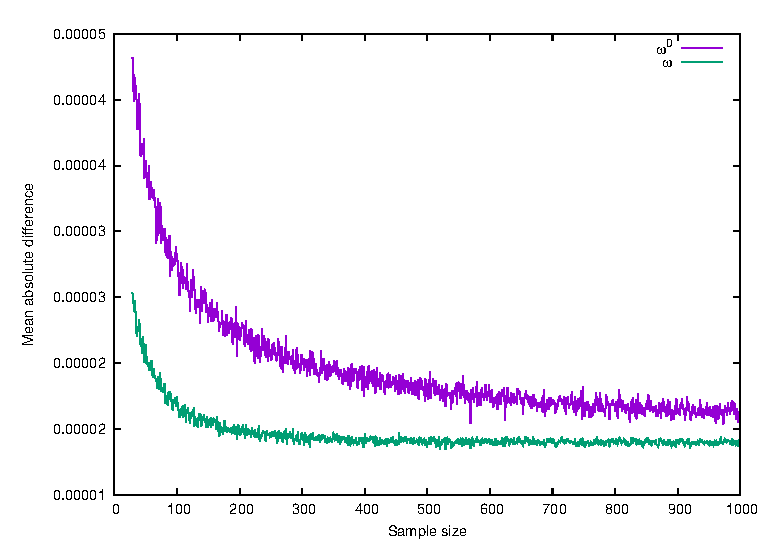
\includegraphics[width=\textwidth]{figs/levmar/comparison/comparison_1000_32_1000_xsigma1.txt_parameter2.eps}
	\caption{$\alpha_0$}
  \end{subfigure}%
  \begin{subfigure}[b]{0.35\textwidth}
    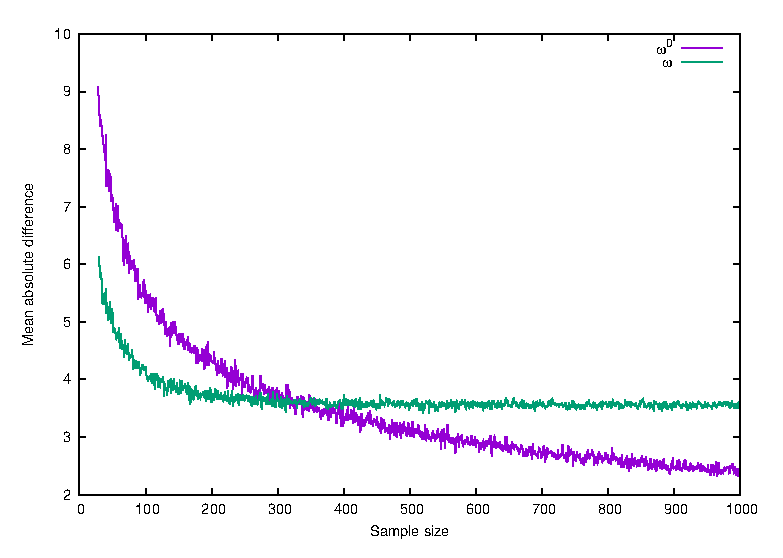
\includegraphics[width=\textwidth]{figs/levmar/comparison/comparison_1000_32_1000_xsigma1.txt_parameter3.eps}
	\caption{$\gamma$}
  \end{subfigure}
  \caption{Сходимость параметров к истинным при $k = 1$.}
  \label{fig:comparison_1}
\end{figure}

\begin{figure}[h]
  \centering
  \begin{subfigure}[b]{0.35\textwidth}
    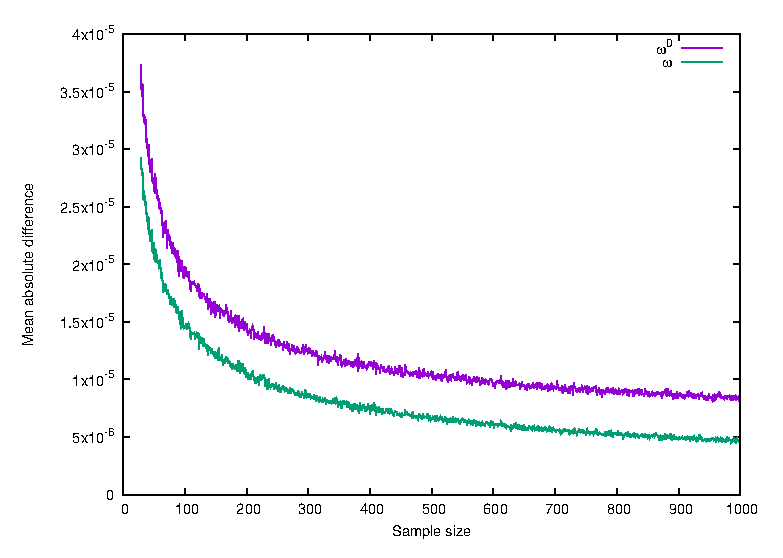
\includegraphics[width=\textwidth]{figs/levmar/comparison/comparison_1000_32_1000_xsigma1.2.txt_parameter1.eps}
	\caption{$g_0$}
  \end{subfigure}%
  \begin{subfigure}[b]{0.35\textwidth}
    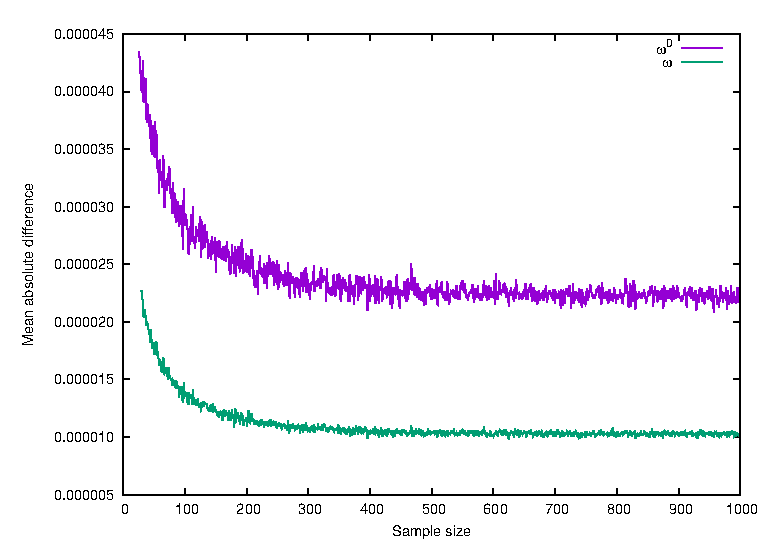
\includegraphics[width=\textwidth]{figs/levmar/comparison/comparison_1000_32_1000_xsigma1.2.txt_parameter2.eps}
	\caption{$\alpha_0$}
	\label{fig:comparison_1.2_alpha}
  \end{subfigure}%
  \begin{subfigure}[b]{0.35\textwidth}
    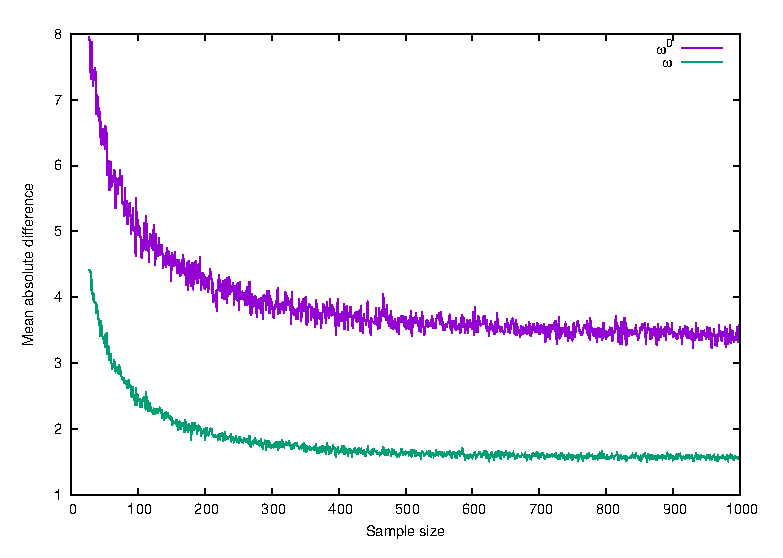
\includegraphics[width=\textwidth]{figs/levmar/comparison/comparison_1000_32_1000_xsigma1.2.txt_parameter3.eps}
	\caption{$\gamma$}
  \end{subfigure}
  \caption{Сходимость параметров к истинным при $k = 1.2$.}
  \label{fig:comparison_1.2}
\end{figure}

\begin{figure}[h]
  \centering
  \begin{subfigure}[b]{0.35\textwidth}
    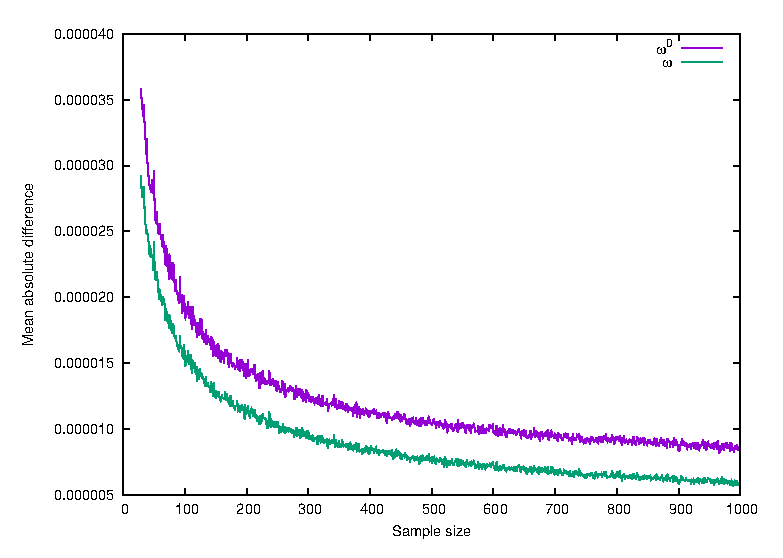
\includegraphics[width=\textwidth]{figs/levmar/comparison/comparison_1000_32_1000_xsigma9.txt_parameter1.eps}
	\caption{$g_0$}
  \end{subfigure}%
  \begin{subfigure}[b]{0.35\textwidth}
    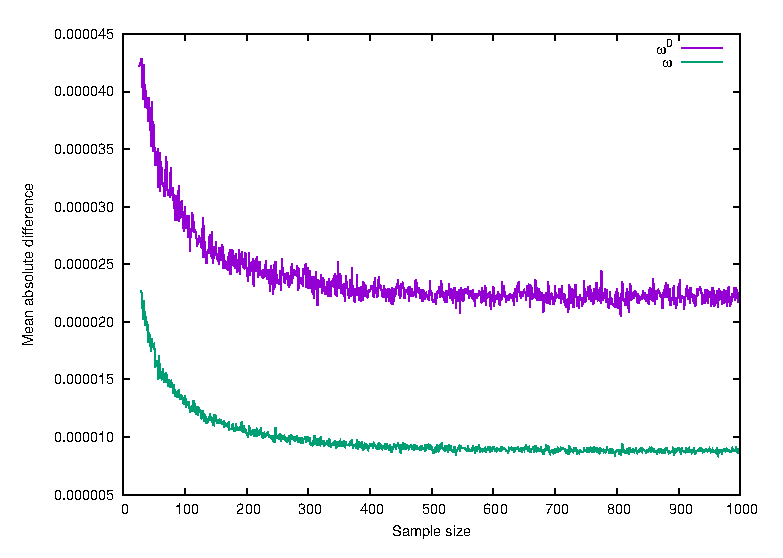
\includegraphics[width=\textwidth]{figs/levmar/comparison/comparison_1000_32_1000_xsigma9.txt_parameter2.eps}
	\caption{$\alpha_0$}
	\label{fig:comparison_9_alpha}
  \end{subfigure}%
  \begin{subfigure}[b]{0.35\textwidth}
    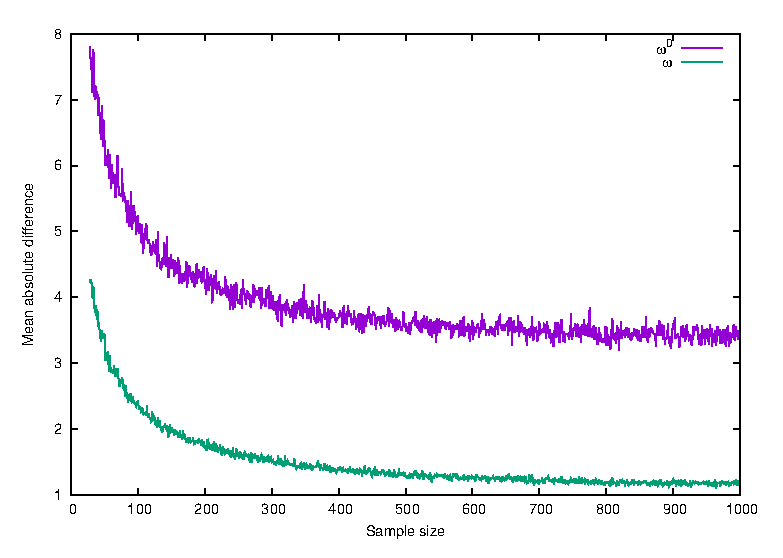
\includegraphics[width=\textwidth]{figs/levmar/comparison/comparison_1000_32_1000_xsigma9.txt_parameter3.eps}
	\caption{$\gamma$}
  \end{subfigure}
  \caption{Сходимость параметров к истинным при $k = 9$.}
  \label{fig:comparison_9}
\end{figure}

\FloatBarrier

\section{Заключение}

Предложен модифицированный функционал среднеквадратичной ошибки для существенно
нелинейных моделей, применимый в случае наличия ошибок измерения независимых
переменных и различия распределения, к которому принадлежат ошибки, в разных
точках обучающей выборки.

Показана сходимость предложенного функционала к классическому функционалу
среднеквадратичной ошибки для случая гомоскедастичности погрешностей
зависимой переменной и пренебрежимо малой погрешности измерения независимых
переменных.

Представляется разумным использовать предложенный в настоящей
работе функционал качества при анализе устойчивости регрессионных моделей к
погрешностям как в зависимых, так и независимых переменных\cite{Rudoy15MonteCarlo,Rudoy16StabilityAnalysis}.

\FloatBarrier

\bibliographystyle{babunsrt-lf}
%\bibliographystyle{babunsrt}
%\bibliographystyle{unsrt}
\bibliography{bibliography}

\end{document}
